\documentclass[11pt]{article}

% ------------------------------
% Packages
% ------------------------------
\usepackage[margin=1in]{geometry}
\usepackage{amsmath, amssymb, amsthm, bbm}
\usepackage{enumitem}
\usepackage{float}
\usepackage{graphicx}
\usepackage{cite}
\usepackage{hyperref}
\usepackage{fancyhdr}
\usepackage{tikz}
\usepackage{lastpage}
\usepackage{xcolor}
\usepackage{array}
\usepackage{multirow}
\usepackage{tabularx}
\usepackage{booktabs}
\usepackage{caption}
\usepackage{minted}
\usepackage{algorithm}
\usepackage{algpseudocode}
\newcolumntype{Y}{>{\raggedright\arraybackslash}X}

% ------------------------------
% Global Settings
% ------------------------------
\setlength{\parindent}{0pt}
\setlength{\parskip}{6pt}
\setlength{\headheight}{14pt}
\hypersetup{
  colorlinks=true,
  linkcolor=blue,
  citecolor=black,
  urlcolor=blue
}
\usetikzlibrary{arrows.meta,positioning}
\usetikzlibrary{shapes.geometric}
\usemintedstyle{friendly}

% ------------------------------
% Metadata
% ------------------------------
\newcommand{\studentName}{Faaiz Khan}
\newcommand{\studentRollNo}{25280051}
\newcommand{\courseCode}{AI600}
\newcommand{\courseName}{Deep Learning}
\newcommand{\hwNumber}{Assignment \#3}
\newcommand{\professorName}{Prof. Dr. Momin Uppal}
\newcommand{\taNames}{Muhammad Aleem Shakeel, Muhammad Usman, Muhammad Qasim Ayub, Usman Ahad}
\newcommand{\dueDate}{Monday April 6, 2026}
\newcommand{\honorPledge}{%
I affirm that I have abided by the academic integrity policy. I have neither given nor received unauthorized aid on this assignment.\\
}

% ------------------------------
% Header & Footer (applies to pages AFTER the cover)
% ------------------------------
\pagestyle{fancy}
\fancyhf{}
\fancyhead[L]{\studentName}
\fancyhead[C]{\courseName}
\fancyhead[R]{\hwNumber}
\fancyfoot[C]{Page \thepage\ of \pageref*{LastPage}}

% ------------------------------
% Problem Environments
% ------------------------------
\newcounter{problem}
\newcounter{task}
\newcounter{question}

% Base "problem" environment: prints bold "Problem n." (optional short title)
\newenvironment{problem}[1][]{
  \refstepcounter{problem}%
  \par\bigskip
  \noindent\textbf{Problem \theproblem.\if\relax\detokenize{#1}\relax\else\ #1\fi}\par
  \medskip
}{\par\bigskip}

\newenvironment{task}[1][]{
  \refstepcounter{task}%
  \par\bigskip
  \noindent{\Large\textbf{Task \thetask:\if\relax\detokenize{#1}\relax\else\ #1\fi}}\par
  \medskip
}{\par}

% Variant that forces a page break at the end:
\newenvironment{problembreak}[1][]{
  \refstepcounter{problem}%
  \par\bigskip
  \noindent\textbf{Problem \theproblem.\if\relax\detokenize{#1}\relax\else\ #1\fi}\par
  \medskip
}{\par\bigskip\clearpage}

\newenvironment{question}[1][]{
  \refstepcounter{question}%
  \par\bigskip
  \noindent{\Large\textbf{Question \thequestion:\if\relax\detokenize{#1}\relax\else\ #1\fi}}\par
  \medskip
}{\par\bigskip}

% ------------------------------
% Document
% ------------------------------
\begin{document}

% -------- Cover Page (no header/footer) --------
\begin{titlepage}
  \thispagestyle{empty}
  \centering
  \vspace*{2cm}
  {\Large \courseCode\ \courseName\par}
  \vspace{0.5cm}
  {\LARGE \hwNumber\par}
  \vspace{0.5cm}
  {\large Due: \dueDate\par}
  \vfill

  \newcolumntype{L}[1]{>{\raggedleft\arraybackslash}m{#1}}
  \newcolumntype{C}[1]{>{\centering\arraybackslash}m{#1}}

  \begin{tabular}{@{} L{0.22\textwidth} C{0.68\textwidth} @{}}
    \textbf{Professor:} & \professorName \\
    \textbf{TA(s):}     & \taNames \\
    \textbf{Student:}   & \studentName \\
    \textbf{Roll No.:}  & \studentRollNo
  \end{tabular}
  
  \vfill

  \begin{minipage}{0.9\textwidth}
    \small
    \textbf{Honor Pledge:}\\[2pt]
    \honorPledge
    \noindent All work, code implementation, and data for this assignment can be found at the following public GitHub repository: \\
\url{https://github.com/FaaizKhan1999/ai600-assignments/tree/main/assignment-02}
    \vspace{1.2cm}
  \end{minipage}
\end{titlepage}

% Start page numbering from 1 after the cover
\setcounter{page}{1}

\section*{Analytical Section}

\subsection*{Section Parameters}

\textbf{Model Architecture Setup:} The 'Toy-CNN' referenced throughout this section is outlined by the computational graph below.

\begin{figure}[H]
  \centering
  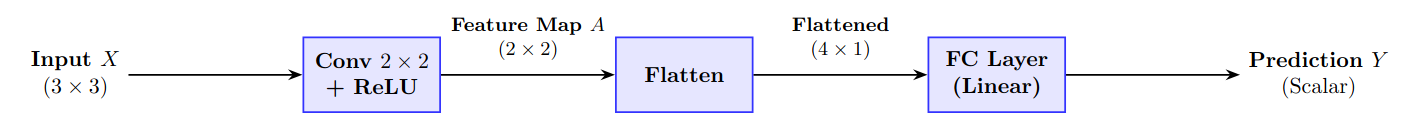
\includegraphics[width=\textwidth]{figs/model-architecture.png}
  \caption{Computational Graph of the 'Toy-CNN'.}
\end{figure}

The input $X$ is a $3 \times 3$ matrix representing a single-channel (grayscale) image.

The first layer is convolutional with a $2 \times 2$ filter $W$, a scalar bias $b$, stride $s=1$, no padding, and ReLU activation.

The second layer is fully connected which initially flattens the output from the first layer into a $4 \times 1$ vector. It comes with a $1 \times 4$ weight vector $V$, a scalar bias $c$, and linear activation.

The loss function is MSE for a single sample: $L=\frac{1}{2} (Y - T)^2$ where $T$ is the true target value.

\textbf{Initial Weights and Data:} The initial weights and data required to perform the forward and/or backward pass are given below.

$$X = \begin{bmatrix}1 & 2 & 0 \\ 0 & 1 & 1 \\ 1 & 0 & 2\end{bmatrix}$$
$$W = \begin{bmatrix}1 & 0 \\ -1 & 1\end{bmatrix}, \qquad b = 0$$
$$V = \begin{bmatrix}1 & -1 & 2 & 0.5\end{bmatrix}, \qquad c = 1$$
$$T = 3$$

\begin{question}[Forward and Backward Pass]
  \textbf{1a) Forward Pass:} Compute the pre-activation feature map $Z$, the post-activation feature
map $A$, the final prediction $Y$, and the loss $L$. (Show all intermediate matrices).
  
  $$Z = X * W + B = \begin{bmatrix}1 & 2 & 0 \\ 0 & 1 & 1 \\ 1 & 0 & 2\end{bmatrix} * \begin{bmatrix}1 & 0 \\ -1 & 1\end{bmatrix} + \begin{bmatrix}0 & 0 \\ 0 & 0\end{bmatrix}$$
  $$Z = \begin{bmatrix}2 & 2 \\ -1 & 3\end{bmatrix} + \begin{bmatrix}0 & 0 \\ 0 & 0\end{bmatrix} = \begin{bmatrix}2 & 2 \\ -1 & 3\end{bmatrix}$$

  $$A = \text{ReLU}(Z) = \begin{bmatrix}\max(0, 2) & \max(0, 2) \\ \max(0, -1) & \max(0, 3)\end{bmatrix} = \begin{bmatrix}2 & 2 \\ 0 & 3\end{bmatrix}$$

  $$Y = V \cdot A_{\text{flattened}} + c = \begin{bmatrix}1 & -1 & 2 & 0.5\end{bmatrix} \cdot \begin{bmatrix}2 \\ 2 \\ 0 \\ 3\end{bmatrix} + 1$$
  $$Y = 1 \cdot 2 + (-1) \cdot 2 + 2 \cdot 0 + 0.5 \cdot 3 + 1 = 2 - 2 + 0 + 1.5 + 1 = 2.5$$

  $$L = \frac{1}{2} (Y - T)^2 = \frac{1}{2} (2.5 - 3)^2 = \frac{1}{2} (0.5)^2=\frac{1}{2} (0.25) = 0.125$$

  \textbf{1b) Backward Pass (Weights):} Compute the gradients of the loss with respect to the fully
  connected weights $(\frac{\partial L}{\partial V})$ and the convolutional filter $(\frac{\partial L}{\partial W})$.

  $$\frac{\partial L}{\partial V} = \frac{\partial L}{\partial Y} \cdot \frac{\partial Y}{\partial V}$$
  $$\frac{\partial L}{\partial V} = (Y - T) \cdot \begin{bmatrix}A_{11} & A_{12} & A_{21} & A_{22}\end{bmatrix} = -0.5 \cdot \begin{bmatrix}2 & 2 & 0 & 3\end{bmatrix}$$
  $$\frac{\partial L}{\partial V} = \begin{bmatrix}-1 & -1 & 0 & -1.5\end{bmatrix}$$

  $$\frac{\partial L}{\partial W} = \frac{\partial L}{\partial Z} \cdot \frac{\partial Z}{\partial W}$$
  $$\frac{\partial L}{\partial Z} = (Y - T) \cdot \left(\begin{bmatrix}V_{11} & V_{12} \\ V_{13} & V_{14}\end{bmatrix} \odot \mathbbm{1}_{x>0}(Z)\right)$$
  $$\frac{\partial L}{\partial Z} = -0.5 \cdot \left(\begin{bmatrix}1 & -1 \\ 2 & 0.5\end{bmatrix} \odot \begin{bmatrix}1 & 1 \\ 0 & 1\end{bmatrix}\right) = -0.5 \cdot \begin{bmatrix}1 & -1 \\ 0 & 0.5\end{bmatrix}$$
  $$\frac{\partial L}{\partial Z} = \begin{bmatrix}-0.5 & 0.5\\ 0 & -0.25\end{bmatrix}$$
  $$\frac{\partial L}{\partial W}_{\text{flattened}} = \begin{bmatrix}1 & 2 & 0 & 1 \\ 2 & 0 & 1 & 1 \\ 0 & 1 & 1 & 0 \\ 1 & 1 & 0 & 2\end{bmatrix} \cdot \begin{bmatrix}-0.5 \\ 0.5 \\ 0 \\ -0.25\end{bmatrix} = \begin{bmatrix}0.25 \\ -1.25 \\ 0.5 \\ -0.5\end{bmatrix}$$
  $$\frac{\partial L}{\partial W} = \begin{bmatrix}0.25 & -1.25 \\ 0.5 & -0.5\end{bmatrix}$$

  \textbf{1c) Interpretation:} Observe the gradient matrix $\frac{\partial L}{\partial W}$. If we were to perform one step of Gradient Descent, which specific weight in the $2 \times 2$ filter $W$ would change the most, and in what direction? Explain structurally why this specific weight has the largest gradient based on the forward pass activations.

  Observing the gradient matrix $\frac{\partial L}{\partial W}$, the weight that would change the most if one step of Gradient Descent is performed is $W_{12}$. Since $\frac{\partial L}{\partial W_{12}} = -1.25$ has the largest absolute magnitude in the matrix, it undergoes the most significant adjustment. The value of the corresponding weight will increase because the gradient is negative.

  Structurally, it can be observed that the ReLU activation kills off $Z_{21}$, so the bottom-left of the feature map is 'dead'. $W_{12}$ is the weight that was paired with the strongest input signal in the region where the model was most active. Therefore, the mismatch between the true and predicted values indicates that $W_{12}$ requires the most tuning.
\end{question}

\refstepcounter{question}

\begin{question}[Pooling and Normalisation]
  \textbf{3a) Max Pooling:} Imagine we replace the flattening step and the $4 \times 1$ fully connected layer with a $2 \times 2$ Global Max Pooling layer applied directly to $A$. The output $Y$ is now simply the maximum value in $A$ (assume bias $c = 0$). Recompute $Y$. How does this architectural change alter the flow of gradients back to $X$ compared to Q1? Which pixels in $X$ now have a gradient of zero?

  If the Global Max Pooling layer is applied directly to $A$, then $Y$ simply becomes the maximum value in $A$, so $Y = 3$ (since $c = 0$). The flow of the gradients now changes drastically since only the component that is involved in the prediction ($A_{22}$) will provide a path to the input when the backpropagation occurs. Therefore, any pixel in $X$ that does not contribute to $A_{22}$ will have zero gradients. Furthermore, within the patch that generates $A_{22}$, the pixel $X_{23}$ also has a zero gradient since its corresponding weight in the filter is 0. In this specific sample, the total gradient is 0 since $Y = T$.

  \textbf{3b) Normalization:} Return to the original architecture, but insert a Layer Normalization step immediately after the ReLU activation, applied to the $2 \times 2$ matrix $A$. Calculate the mean $\mu$ and variance $\sigma^2$ of $A$, and write out the normalized feature map $A_\text{norm}$ (assume scale $\lambda = 1$, shift $\beta = 0$, and $\epsilon = 0$ for simplicity).

  $$\mu = \frac{2 + 2 + 0 + 3}{4} = 1.75$$
  
  $$\sigma^2 = \frac{(2 - 1.75)^2 + (2 - 1.75)^2 + (0 - 1.75)^2 + (3 - 1.75)^2}{4} = \frac{0.25^2 + 0.25^2 + (-1.75)^2 + 1.25^2}{4}$$
  $$\sigma^2 = 1.1875 \Longrightarrow \sigma = 1.090$$

  $$A_{\text{norm}} = \begin{bmatrix}0.229 & 0.229 \\ -1.606 & 1.147\end{bmatrix}$$

  \textbf{3c) Interpretation:} Max pooling is often said to provide “translation invariance.” Based on your calculations in 3a, explain mathematically why shifting the input image $X$ slightly to the left or right might not change the output $Y$ or the resulting loss.
  
  If the image is shifted slightly in any direction, it might not change the output $Y$ or the resulting loss since the convolution filter will still return similar values yielded previously, just with changed indices in the feature map. Once Max Pooling is applied to the feature map, due to its commutativity and associativity, the prediction will remain the same.
\end{question}

\pagebreak

\section*{Programming: Implementation and Analysis}

\begin{task}[Custom CNNs and Shortcut Learning]
  \textbf{Part A: Standard MNIST}

  \textbf{1. Architecture Design:} A custom CNN was implemented with 3 convolutional layers and 2 fully connected linear layers. The total number of trainable parameters were 25,706 adhering to the constraint set.

  \textbf{2. Training and Evaluation:} The model was trained using the Adam optimizer and Cross-Entropy loss. The training and validation loss and accuracy over the epochs is plotted in the figure below.

  \begin{figure}[H]
    \centering
    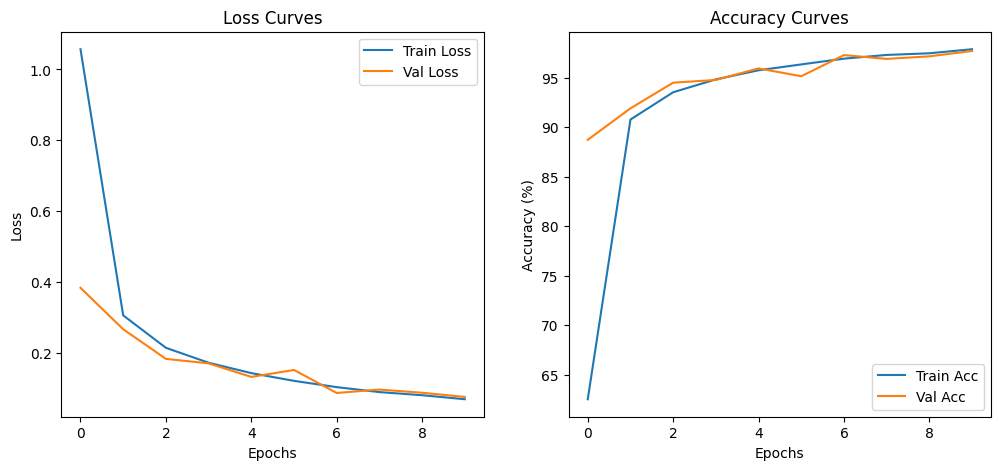
\includegraphics[scale=0.6]{figs/loss-accuracy-curves.png}
    \caption{MNIST Dataset Training and Validation Loss and Accuracy Curves.}
  \end{figure}

  As can be seen from the image, the training and validation accuracies reach a near perfect score around 98\% after 10 epochs. The model is evaluated on the test set and reaches an accuracy of 97.92\%.

  \textbf{3. Analytical Question 1.1:} The model generalises adequately as can be seen from the equally high accuracies among the three sets. There is also no gap in the losses of the training and validation sets.

  \textbf{4. Analytical Question 1.2:} The weights of the 16 filters present in the first convolutional layer are extracted and plotted as images below.

  \begin{figure}[H]
  \centering
  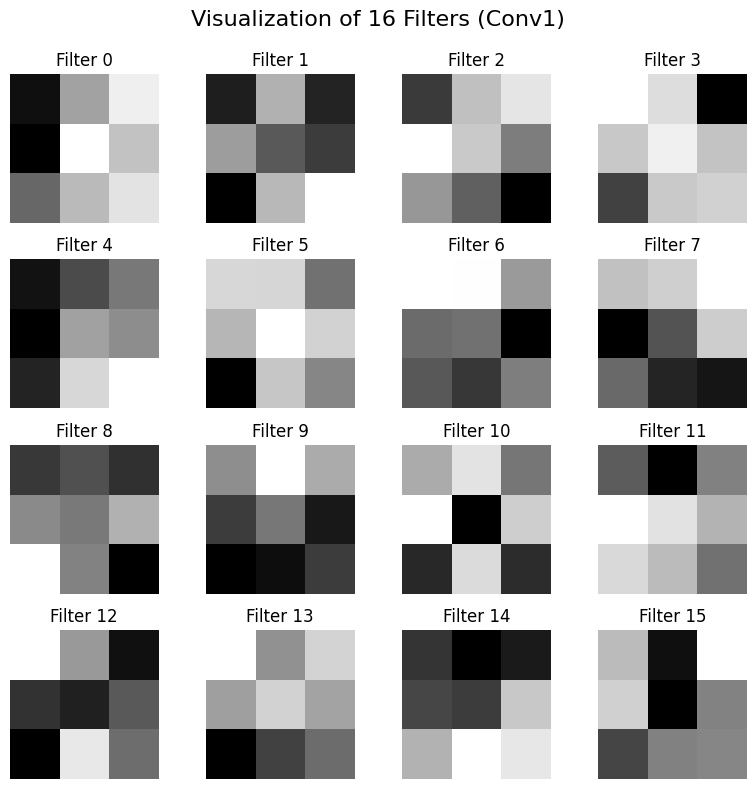
\includegraphics[scale=0.6]{figs/filter-visualisation.png}
  \caption{Filter Visualisations from the First Convolutional Layer.}
  \end{figure}

  These plots already point to some rudimentary edge/texture detection. For example, filters 1 and 4 may be used to detect vertical edges due to the presence of a dark column. Likewise, filters 9 and 14 may be used as horizontal edge detectors and filters 10 and 12 as diagonal edge detectors. These filters seem to capture spatial gradients, including edges, textures, and orientations.

  \textbf{Part B: Coloured-MNIST (CMNIST)}

  \textbf{1. Adaptation:} The model used in Part A was simply modified to take in 3 input channels instead of 1. This was then trained on the biased training set provided.

  \textbf{2. Evaluation:} The model was then evaluated on both the biased and unbiased training sets.

  \textbf{3. Analytical Question 1.3:} The biased test set yielded an accuracy of 97.16\% whereas the unbiased test set showed a significant drop in accuracy with only 47.54\%. This is because it found a shortcut in the data. In the biased training set, color may have been a near-perfect predictor of the digit's label, and since neural networks are designed for Empirical Risk Minimisation, the optimizer naturally prioritized the simplest path to reducing loss. Mathematically, the gradient for a simple feature like color is much stronger and more direct than the complex, non-linear gradients required to learn the geometry of a shape through multiple convolutional layers. Conceptually, this is known as Shortcut Learning: the model becomes "lazy" and ignores the difficult shape features in favor of the easy color features.

  \textbf{4. Analytical Question 1.4:} The most obvious training strategy that would improve the result is data augmentation: specifically colour jittering, making sure that the colours remain as unbiased as possible throughout the training set. This forces the model to focus more on the shape rather than the colour of the images. Other strategies may include Domain Adversarial Training or Strategic Spectral Decoupling.
\end{task}

\begin{task}[Transfer Learning and Interpretability]
  \textbf{Part A: Fine-Tuning ResNet-18}

  \textbf{1. Model Setup:} The model was successfully loaded using \texttt{torchvision.models}.
  
  \textbf{2. Freezing the Backbone:} All the convolutional layers of the model were frozen, making it so their gradients are not computed during the backpropagation.

  \textbf{3. Classification Head:} The final layer was replaced with a layer that outputs 10 classes matching the STL-10 dataset that the model is being trained on.

  \textbf{4. Training:} The model was trained on the training set and then evaluated on the test set, yielding an accuracy of 94.45\%.

  \textbf{5. Analytical Question 2.1:} Freezing the early layers of a pre-trained network is beneficial because those layers act as a universal feature extractor that has already learned to identify basic visual building blocks like edges, corners, and simple textures. These low-level features are a commonality in all images, so they don't need to be relearned for a new dataset. Computationally, this saves a chunk of time and memory because the optimizer only has to calculate gradients and update weights for the final classification head rather than all 11 million parameters. Functionally, since the labeled STL-10 dataset is relatively small, freezing the convolutional layer prevents overfitting, where a powerful model might accidentally memorize the specific noise or background of the small training set instead of learning generalizable patterns. While the early layers capture these simple geometric primitives, the later layers store high-level features such as the distinct shape of a bird's wing or the structure of a truck.

  \textbf{Part B: Visualising Decisions with GradCAM}

  \textbf{1. Implementation:} GradCAM was imported using an existing library and the activations maps were extracted from the final convolutional layer of the fine-tuned model.

  \textbf{2. Visualisation:} The 2 correctly and 2 incorrectly labelled images are provided below.

  \begin{figure}[H]
    \centering
    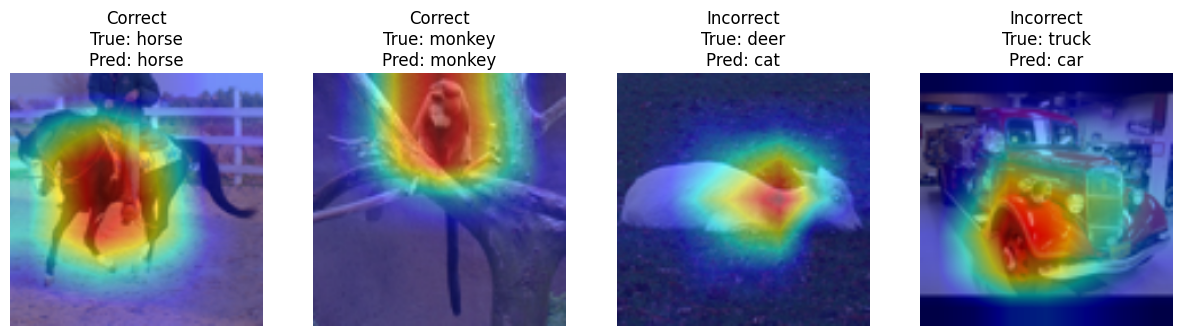
\includegraphics[width=\textwidth]{figs/labelled-images.png}
    \caption{Correctly and Incorrectly Labelled STL-10 Images.}
  \end{figure}

  \textbf{3. Analytical Question 2.2:} Analysing the heatmaps of the correctly classified images, it can be seen that the model is correctly honing in on the object that it needs to focus on to make the prediction. Often times, this object may not be centered but the model is smart enough to ignore all the noise and complete the task at hand with relatively hgih accuracy.

  \textbf{4. Analytical Question 2.3:} For the images it does mislabel, it can be observed that the model is only focused on part of the object or a local feature. This tunnel-vision makes it so it mislabels are truck by classifying it as a car or a goat by saying it is a cat.

\end{task}
\pagebreak

{\Large\textbf{GEN AI USAGE}}\\[1em]
All the content written in the report is written explicitly by me. Gen AI tools were only ever used as an aid for conceptual understanding and had no direct role in solving the questions. All research related to decision-making and understanding was also done by me.\\
The relevant content pertaining to the assignment was also written by myself. VS Code's Copilot was used to help provide boilerplate code instead of writing any of the logic.

\end{document}
